

Voici le tableau de variations de la fonction $f$.

\begin{tikzpicture}
\tkzTabInit[lgt=1,espcl=2]{ $x$ / 1,$f $ / 2}
{ $-4$ , $-1$ ,1,5}
\tkzTabVar{-/$-5$,+/$3$,-/$-1$,+/$5$ }
\end{tikzpicture}
\begin{enumerate}
\item Comparer $f(2)$ et $f(4)$.

2 et 4 appartiennent à l'intervalle $[1;5]$ sur lequel la fonction $f$ est croissante. 

$2<4$ donc $f(2)<f(4)$


\item Trace une courbe qui représente cette fonction $f$.


\definecolor{qqqqqq}{rgb}{0.,0.,0.}
\definecolor{ududff}{rgb}{0.30196078431372547,0.30196078431372547,1.}
\begin{tikzpicture}[line cap=round,line join=round,>=triangle 45,x=1.0cm,y=1.0cm]
\begin{axis}[
x=1.0cm,y=1.0cm,
axis lines=middle,
ymajorgrids=true,
xmajorgrids=true,
xmin=-5.68,
xmax=5.94,
ymin=-5.299999999999999,
ymax=5.699999999999999,
xtick={-5.0,-4.0,...,5.0},
ytick={-5.0,-4.0,...,5.0},]
\clip(-5.68,-5.3) rectangle (5.94,5.7);
\draw [line width=4.pt] (-1.06,2.98)-- (-1.06,2.98)-- (-1.12,2.94)-- (-1.18,2.88)-- (-1.26,2.82)-- (-1.34,2.74)-- (-1.4,2.72)-- (-1.44,2.66)-- (-1.5,2.62)-- (-1.56,2.58)-- (-1.62,2.5)-- (-1.68,2.46)-- (-1.74,2.4)-- (-1.8,2.36)-- (-1.82,2.3)-- (-1.84,2.24)-- (-1.9,2.18)-- (-1.96,2.12)-- (-1.98,2.06)-- (-2.02,2.)-- (-2.08,1.94)-- (-2.14,1.86)-- (-2.18,1.8)-- (-2.24,1.72)-- (-2.3,1.66)-- (-2.32,1.6)-- (-2.36,1.54)-- (-2.4,1.46)-- (-2.44,1.4)-- (-2.48,1.32)-- (-2.54,1.3)-- (-2.58,1.24)-- (-2.6,1.18)-- (-2.66,1.12)-- (-2.7,1.)-- (-2.72,0.94)-- (-2.76,0.88)-- (-2.78,0.82)-- (-2.8,0.76)-- (-2.84,0.7)-- (-2.88,0.62)-- (-2.9,0.52)-- (-2.96,0.44)-- (-2.98,0.36)-- (-3.02,0.3)-- (-3.02,0.2)-- (-3.02,0.12)-- (-3.06,0.04)-- (-3.06,-0.04)-- (-3.12,-0.1)-- (-3.12,-0.18)-- (-3.16,-0.28)-- (-3.18,-0.34)-- (-3.22,-0.44)-- (-3.22,-0.56)-- (-3.26,-0.62)-- (-3.3,-0.68)-- (-3.32,-0.76)-- (-3.34,-0.84)-- (-3.34,-0.92)-- (-3.36,-0.98)-- (-3.42,-1.06)-- (-3.42,-1.14)-- (-3.44,-1.2)-- (-3.46,-1.26)-- (-3.48,-1.36)-- (-3.5,-1.44)-- (-3.5,-1.54)-- (-3.52,-1.62)-- (-3.52,-1.7)-- (-3.56,-1.76)-- (-3.6,-1.86)-- (-3.62,-1.92)-- (-3.64,-2.02)-- (-3.66,-2.12)-- (-3.68,-2.2)-- (-3.72,-2.26)-- (-3.74,-2.32)-- (-3.76,-2.4)-- (-3.78,-2.48)-- (-3.8,-2.54)-- (-3.8,-2.62)-- (-3.8,-2.72)-- (-3.82,-2.8)-- (-3.86,-2.86)-- (-3.86,-2.96)-- (-3.86,-3.04)-- (-3.9,-3.1)-- (-3.9,-3.18)-- (-3.9,-3.26)-- (-3.92,-3.32)-- (-3.94,-3.38)-- (-3.94,-3.46)-- (-3.96,-3.52)-- (-4.,-3.64)-- (-4.,-3.74)-- (-4.,-3.82)-- (-4.,-3.9)-- (-4.02,-3.96)-- (-4.02,-4.06)-- (-4.02,-4.14)-- (-4.02,-4.24)-- (-4.02,-4.36)-- (-4.04,-4.42)-- (-4.04,-4.5)-- (-4.04,-4.62)-- (-4.04,-4.72)-- (-4.04,-4.8)-- (-4.04,-4.88)-- (-4.04,-4.96)-- (-4.02,-5.02);
\draw [line width=4.pt] (-0.92,3.02)-- (-0.92,3.02)-- (-0.94,2.96)-- (-0.94,2.88)-- (-0.94,2.78)-- (-0.92,2.72)-- (-0.9,2.66)-- (-0.88,2.58)-- (-0.84,2.52)-- (-0.82,2.44)-- (-0.82,2.34)-- (-0.8,2.28)-- (-0.8,2.18)-- (-0.78,2.12)-- (-0.78,2.04)-- (-0.76,1.98)-- (-0.76,1.88)-- (-0.74,1.8)-- (-0.74,1.72)-- (-0.74,1.6)-- (-0.68,1.5)-- (-0.68,1.4)-- (-0.66,1.34)-- (-0.66,1.22)-- (-0.64,1.16)-- (-0.62,1.08)-- (-0.62,1.)-- (-0.6,0.92)-- (-0.58,0.86)-- (-0.54,0.78)-- (-0.52,0.7)-- (-0.5,0.62)-- (-0.48,0.54)-- (-0.46,0.44)-- (-0.46,0.36)-- (-0.4,0.3)-- (-0.38,0.24)-- (-0.36,0.16)-- (-0.34,0.1)-- (-0.32,0.02)-- (-0.3,-0.04)-- (-0.24,-0.06)-- (-0.22,-0.12)-- (-0.18,-0.18)-- (-0.12,-0.24)-- (-0.06,-0.28)-- (-0.04,-0.34)-- (0.,-0.4)-- (0.06,-0.46)-- (0.12,-0.5)-- (0.18,-0.54)-- (0.24,-0.6)-- (0.3,-0.64)-- (0.36,-0.68)-- (0.44,-0.7)-- (0.5,-0.76)-- (0.56,-0.78)-- (0.62,-0.8)-- (0.7,-0.82)-- (0.76,-0.88)-- (0.82,-0.9)-- (0.88,-0.94)-- (0.94,-0.96)-- (1.,-0.98)-- (0.94,-0.94);
\draw [line width=4.pt,color=qqqqqq] (4.96,4.94)-- (4.96,4.94)-- (4.86,4.9)-- (4.76,4.9)-- (4.68,4.9)-- (4.58,4.88)-- (4.5,4.86)-- (4.4,4.82)-- (4.28,4.82)-- (4.18,4.8)-- (4.12,4.78)-- (4.06,4.74)-- (3.96,4.74)-- (3.92,4.68)-- (3.8,4.62)-- (3.72,4.6)-- (3.64,4.54)-- (3.58,4.52)-- (3.5,4.48)-- (3.44,4.46)-- (3.4,4.4)-- (3.34,4.36)-- (3.3,4.28)-- (3.22,4.22)-- (3.14,4.16)-- (3.08,4.1)-- (3.,4.02)-- (2.94,3.94)-- (2.88,3.88)-- (2.82,3.8)-- (2.78,3.74)-- (2.72,3.7)-- (2.66,3.64)-- (2.6,3.58)-- (2.56,3.5)-- (2.5,3.42)-- (2.48,3.36)-- (2.42,3.3)-- (2.38,3.24)-- (2.34,3.18)-- (2.26,3.1)-- (2.22,3.04)-- (2.22,2.96)-- (2.16,2.88)-- (2.14,2.8)-- (2.1,2.74)-- (2.06,2.64)-- (2.02,2.56)-- (1.92,2.46)-- (1.9,2.4)-- (1.88,2.32)-- (1.88,2.22)-- (1.8,2.08)-- (1.78,1.98)-- (1.72,1.88)-- (1.72,1.8)-- (1.7,1.72)-- (1.7,1.62)-- (1.64,1.54)-- (1.64,1.46)-- (1.62,1.36)-- (1.62,1.26)-- (1.62,1.18)-- (1.6,1.12)-- (1.6,1.04)-- (1.58,0.96)-- (1.58,0.86)-- (1.56,0.8)-- (1.54,0.72)-- (1.54,0.64)-- (1.52,0.58)-- (1.5,0.46)-- (1.48,0.4)-- (1.46,0.34)-- (1.46,0.26)-- (1.44,0.18)-- (1.42,0.1)-- (1.4,0.04)-- (1.36,-0.04)-- (1.34,-0.12)-- (1.32,-0.18)-- (1.3,-0.24)-- (1.28,-0.3)-- (1.26,-0.36)-- (1.22,-0.42)-- (1.2,-0.48)-- (1.18,-0.56)-- (1.16,-0.62)-- (1.14,-0.68)-- (1.12,-0.74)-- (1.08,-0.82)-- (1.06,-0.92)-- (1.06,-1.);
\begin{scriptsize}
\draw [color=ududff] (-4.,-5.)-- ++(-2.5pt,0 pt) -- ++(5.0pt,0 pt) ++(-2.5pt,-2.5pt) -- ++(0 pt,5.0pt);
\draw[color=ududff] (-3.86,-4.63) node {$A$};
\draw [color=ududff] (-1.,3.)-- ++(-2.5pt,0 pt) -- ++(5.0pt,0 pt) ++(-2.5pt,-2.5pt) -- ++(0 pt,5.0pt);
\draw[color=ududff] (-0.86,3.37) node {$B$};
\draw [color=ududff] (1.,-1.)-- ++(-2.5pt,0 pt) -- ++(5.0pt,0 pt) ++(-2.5pt,-2.5pt) -- ++(0 pt,5.0pt);
\draw[color=ududff] (1.26,-1.07) node {$C$};
\draw [color=ududff] (5.,5.)-- ++(-2.5pt,0 pt) -- ++(5.0pt,0 pt) ++(-2.5pt,-2.5pt) -- ++(0 pt,5.0pt);
\draw[color=ududff] (5.14,5.37) node {$D$};
\end{scriptsize}
\end{axis}
\end{tikzpicture}




\item Pour quelle valeur de $x$, $f(x)$ est minimal ? Que vaut ce minimum ?

D'après le tableau de variations, $f$ admet un minimal égal à $-5$ atteint pour $x=-4$.

\item Est-il vrai que $f(x)=0$ admet une solution ? Justifier.

 $f(x)=0$ n'admet pas une solution mais plusieurs solutions sur son domaine de définition. $f(x)=0$ admet exactement 3 solutions sur $[-4;5]$
 


\begin{tikzpicture}
\tkzTabInit[lgt=1,espcl=2]{ $x$ / 1,$f $ / 2}
{ $-4$ , $-1$ ,1,5}
\tkzTabVar{-/$-5$,+/$3$,-/$-1$,+/$5$ }
\tkzTabVal{1}{2}{0.5}{}{0}
\tkzTabVal{2}{3}{0.5}{}{0}
\tkzTabVal{3}{4}{0.5}{}{0}
\end{tikzpicture}


\end{enumerate}
